% TACL submission, generated by html2tex (tacl template).
% Official style: tacl2021v1.sty (https://transacl.org/tacl-submission-templates/).
\documentclass[11pt,a4paper]{article}
\usepackage{times,latexsym}
\usepackage{url}
\usepackage[T1]{fontenc}

% SUBMISSION version: tacl2021v1 (no option) gives two-column A4, Times 11pt,
% margin line numbers (native lineno, no overlap), and the "Confidential TACL
% submission" header. For CAMERA-READY, switch to [acceptedWithA] (drops the
% line numbers + header and reveals authors).
\usepackage[]{tacl2021v1}
%\usepackage[acceptedWithA]{tacl2021v1}

\usepackage{hyperref}

% Shared html2tex compatibility preamble (tables, floats, graphics,
% verbatim, pandoc helper macros, numeric citations). One \input keeps
% every venue template in sync with the accumulated compile fixes.
% html2tex compatibility preamble (shared across ALL venue templates).
%
% This file collects every package load and macro provider that makes
% pandoc's HTML->LaTeX output compile cleanly under a venue's own style
% file. Each venue template (templates/<venue>/main.tex.template) should
% \input this file AFTER it loads its own \documentclass + venue .sty,
% and BEFORE \begin{document}. pack_tmlr_bundle.py copies this file into
% every bundle, so a new venue template inherits all accumulated fixes
% by adding a single \input line.
%
% Every entry below is load-bearing for a specific pandoc construct; the
% comment names the construct and the failure it prevents. Do NOT remove
% one without checking the matching post-processor rule in
% convert_to_tex.py.

% --- Captions / float numbering --------------------------------------
% The source HTML numbers its floats itself ("Table 8E", "Figure 5") in
% BOTH the prose and the caption text. LaTeX's automatic float counter
% counts differently (1..N in float order), which would desync caption
% numbers from the prose cross-references. Suppress the automatic
% "Table N:" / "Figure N:" label so the HTML's own number (kept in the
% caption text) is the single source of truth and always matches prose.
\usepackage{caption}
\captionsetup{labelformat=empty,labelsep=none,skip=4pt}

% --- Tables -----------------------------------------------------------
% tabularx + array: convert_to_tex.py rewrites pandoc longtable blocks to
% weighted tabularx so wide text wraps and columns are content-sized.
\usepackage{tabularx}
\usepackage{array}
% longtable: page-breakable tables. convert_to_tex.py emits tall
% verbatim-bearing tables (side-by-side review examples) as longtable so
% they split across pages instead of overrunning a single page / float.
\usepackage{longtable}
% booktabs: \toprule / \midrule / \bottomrule used by every converted table.
\usepackage{booktabs}

% --- Floats -----------------------------------------------------------
% float provides the [H] "put it exactly HERE, do not float" specifier.
% convert_to_tex.py places figures and (single-column) tables with [H] so
% they appear right where the source HTML put them -- right after their
% "Figure N shows..." sentence -- instead of floating off and (a)
% splitting a sentence across the float, (b) drifting into the
% references, or (c) leaving a near-blank page. In two-column mode a wide
% table still floats full-width ([t]) because [H] full-width is illegal.
\usepackage{float}
% placeins / \FloatBarrier kept available for any manual use, though the
% [H] policy means convert_to_tex.py no longer inserts barriers.
\usepackage{placeins}
% \raggedbottom is REQUIRED with the [H] float policy. Many venue styles
% (tmlr.sty does, line "\flushbottom \sloppy") force \flushbottom, which
% vertically JUSTIFIES every page -- it stretches the glue around section
% headings and floats so each page is exactly full. When an [H] float
% does not fit and moves to the next page, the current page is under-full
% and \flushbottom stretches it, producing large gaps ("heading at top,
% blank middle, text at bottom"; "gap after a table"). \raggedbottom
% lets pages end naturally instead. Set both directly (this file is
% \input AFTER the venue \flushbottom) and \AtBeginDocument (in case the
% class re-asserts \flushbottom at begin-document), so it always wins.
\raggedbottom
\AtBeginDocument{\raggedbottom}

% Tighten the vertical gap around floats. Under the [H] policy a figure/table
% is set inline, so the space below its caption is \intextsep; LaTeX's ~12pt
% default reads as two blank lines after the caption. ~6pt is one clean line.
% \textfloatsep / \floatsep cover the full-width table* floats that still
% float to the column/page top. One change, every float and caption.
\setlength{\intextsep}{6pt plus 2pt minus 2pt}
\setlength{\textfloatsep}{8pt plus 2pt minus 2pt}
\setlength{\floatsep}{8pt plus 2pt minus 2pt}

% Never hyphenate cross-reference words: a broken "Fig-ure 2" / "Ta-ble 3"
% reads as an error, not a line break. A word listed with no discretionary
% hyphens is forbidden from breaking.
\hyphenation{Figure Figures Table Tables Appendix Appendices Section Sections}

% --- Graphics ---------------------------------------------------------
% graphicx: SVG figures are pre-rasterized to PDF (svglib) and referenced
% via \includegraphics{X.pdf}.
\usepackage{graphicx}
% xcolor: needed for the `black!75!blue` link-color mixing below (plain
% `color`, which hyperref loads, lacks the `!` mix syntax).
\usepackage{xcolor}
% svg: fallback only. We normally rewrite \includesvg{X.svg} ->
% \includegraphics{X.pdf}, but keep the package so a residual
% \includesvg (e.g. an SVG svglib could not convert) still compiles where
% Inkscape is available (Overleaf). Harmless when unused.
\usepackage{svg}
\svgsetup{inkscapelatex=false}

% --- Verbatim ---------------------------------------------------------
% fvextra extends fancyvrb with the `breaklines`/`breakanywhere` options
% that the base package lacks. convert_to_tex.py rewrites pandoc's plain
% \begin{verbatim} to \begin{Verbatim}[breaklines=true,breakanywhere=true]
% so long prompt/JSON/code lines WRAP instead of overflowing the page
% (the lmtt overfull-hbox warnings). Tables that contain a verbatim block
% are emitted as plain `tabular` (not tabularx, which double-scans its
% body and forbids verbatim).
\usepackage{fvextra}

% --- Math -------------------------------------------------------------
\usepackage{amsmath}
\usepackage{amssymb}

% --- Typographic quality ---------------------------------------------
% microtype: character protrusion + font expansion. Markedly improves
% justification, kills most overfull \hbox warnings, and is the single
% biggest "looks like a real paper" win. Guard the load so a venue that
% already loads it (or a non-pdftex engine) does not error.
\usepackage{microtype}
% Sensible link colors instead of hyperref's default garish boxes/reds.
% hyperref is loaded by the venue template BEFORE this file, so configure
% it here. Guard with \@ifpackageloaded so venues without hyperref skip.
\makeatletter
\@ifpackageloaded{hyperref}{%
  \hypersetup{%
    colorlinks=true,%
    linkcolor={black!75!blue},%
    citecolor={black!70!green},%
    urlcolor={black!60!blue},%
    breaklinks=true%
  }%
}{}
\makeatother

% --- Pandoc helper macros --------------------------------------------
% Pandoc defines these in its own default template; we ship our own
% template, so we provide them. \tightlist collapses spacing in lists
% pandoc marks "tight"; \passthrough wraps inline verbatim.
\providecommand{\tightlist}{\setlength{\itemsep}{0pt}\setlength{\parskip}{0pt}}
\providecommand{\passthrough}[1]{#1}
% Typographic character macros pandoc emits (would otherwise need
% textcomp, which can clash with venue fonts). Provide inline.
\providecommand{\textquotesingle}{\char39}
\providecommand{\textasciigrave}{\char96}
% Pandoc longtable width helper (only appears if a longtable slips past
% the rewriter); make it a no-op multiplier so it never crashes.
\providecommand{\real}[1]{#1}

% --- Citations --------------------------------------------------------
% Citation STYLE is venue-specific and therefore NOT set here (this file is
% shared by every venue). A numeric venue (TMLR, IEEE) sets
% \setcitestyle{numbers,square,comma} in its own main.tex.template AFTER this
% \input, paired with convert_to_tex.py --citations numeric (numeric \bibitem
% + [N] links). An author-year venue (TACL/ACL) sets nothing -- natbib's
% author-year default stands -- paired with --citations author-year
% (\bibitem[Author(Year)]{key} + \citep/\citet), which those venues REQUIRE
% (numeric citations are a desk-reject violation there).


% Vertical-justification policy is venue-specific and pairs with the float
% policy. This is a TWO-COLUMN venue: convert_to_tex.py --columns 2 floats
% figures/tables with [tbp] (never [H]), so they fill columns instead of
% leaving holes. With floating floats, \flushbottom justifies every page to
% full height (the dense, gap-free standard ACL look) WITHOUT the [H]-float
% glue-stretch gaps. This overrides the compat default \raggedbottom, which is
% correct only for single-column [H] venues (TMLR). \AtBeginDocument wins over
% the compat's same-hook \raggedbottom.
\flushbottom
\AtBeginDocument{\flushbottom}

\title{CoEval: Ranking Language Models for Custom Tasks Without Labeled Data or Trustworthy Benchmarks}

% Anonymous for TACL's double-blind review. For camera-ready, replace with the
% real author block (see tacl2021v1-template.tex for the two formatting options).
\author{Anonymous Authors \\ Anonymous Affiliations}

\date{}

\begin{document}
\maketitle

\begin{abstract}
Selecting a pretrained language model, or evaluating a fine-tuned one, for a specific application is a high-value decision, yet the public benchmarks used to make it are poorly suited: a generic benchmark need not reflect a particular sub-domain, and its scores are suspect once its items leak into pretraining and are recalled rather than solved. We present CoEval, an open framework that supplies a trustworthy, task-specific signal through ensemble self-evaluation. From a task or domain description, a pool of models rotates through all three roles, teacher, student, and judge, generating a fresh contamination-free benchmark, answering it, and scoring one another with no human labels. Because every model also answers as a student, the responses weight each question by its discriminative power and each judge by its consensus with the panel. Where ground truth exists, CoEval recovers the true ranking, tracks objective correctness at $\rho = 0.86$, and reproduces the gold ranking of thirteen models at Spearman $0.95$; on standard meta-evaluation benchmarks (SummEval, LLMBar) the panel matches the best single judge without a label-oracle to select it. Reliability comes from panel composition, not size. Generated items show zero verbatim overlap with five public benchmarks, the panel cancels verbosity bias and same-family self-preference, and rankings are domain-specific. The same pipeline reruns on each model release, giving any team a contamination-free leaderboard for its application.
\end{abstract}

\section{Introduction}\label{introduction}

A practitioner selecting a pretrained language model, or evaluating a fine-tuned one, for a specific application
(summarizing clinical notes, answering over an internal knowledge base, triaging support tickets) faces a deceptively
simple question: \emph{which model is best for my use case?} Answering it well needs an evaluation set that reflects
that use case, and the static, human-curated benchmarks that dominate LLM evaluation make this hard in three ways. They
are \emph{non-extensible} (covering a new domain or difficulty band needs fresh, slow annotation, and for a
proprietary domain the data may not exist at all); \emph{contamination-prone} (public items leak into pretraining
corpora, so a high score can reflect memorization rather than capability \citep{ref12, ref13}); and \emph{generic} (an average-case distribution rarely matches the inputs, scoring criteria,
or edge cases of a particular system). When a practitioner has neither task-specific labeled data \emph{nor} a
benchmark they can trust, they are stuck. \textbf{CoEval} is built for exactly this situation: it generates a
fresh, domain-targeted evaluation from a task description and ranks candidate models on it, with no labels and no
contaminated items.

LLM-as-judge evaluation \citep{ref1, ref2} addresses the cost and extensibility of scoring,
grading free-form responses against a rubric at a fraction of human cost, but a single judge is not a neutral
instrument: judges exhibit positional, \emph{verbosity} \citep{ref8}, and \emph{self-preference} biases,
and a measurement built on one biased instrument inherits its distortions.

We argue that both problems, the rigidity of static benchmarks and the bias of single judges, are best
solved together, by a system that \emph{generates} the evaluation set as carefully as it \emph{scores} it. We
present \textbf{CoEval}, a declarative and reproducible framework for \emph{ensemble self-evaluation}: a
pool of models rotates through all three roles, \emph{teacher}, \emph{student}, and \emph{judge}, to generate a
fresh, contamination-free benchmark, answer it, and score one another. Because every model also answers as a student,
the responses provide the data that weight each question by its discriminative power and each judge by its consensus
with the panel. CoEval contributes:

\begin{itemize}
\tightlist
\item
  \textbf{(1) Self-generating, contamination-resistant benchmarks.} A teacher model synthesizes an
  attribute-stratified benchmark targeted at a declared domain. Because items are freshly generated per run, they
  are resistant to leakage into a student\textquotesingle s training data by construction, and the generated items are
  \emph{discriminative}, separating candidate models (most carry ranking signal), the property a benchmark needs to
  rank them rather than saturate.
\item
  \textbf{(2) A self-validating cross-family judge panel: composition over size.} Responses are scored by
  judges drawn from distinct model vendors. Our central finding is that \emph{composition} (vendor diversity), not
  panel \emph{size}, is the decisive reliability lever: adding low-agreement judges can \emph{reduce} reliability, a
  result that reframes how judge panels should be assembled. Crucially, the panel also \emph{audits itself}: a judge\textquotesingle s
  agreement with the rest is a label-free estimate of its reliability, so the ensemble detects and down-weights broken
  judges (a random, constant, or anti-correlated judge is driven to zero weight) with no ground truth, something a
  single judge cannot do.
\item
  \textbf{(3) Bias-cancelling aggregation.} Consensus aggregation across a vendor-diverse panel cancels
  verbosity bias that individual judges carry with mixed sign, and the vendor-disjoint design structurally precludes
  same-family self-preference.
\item
  \textbf{(4) A reusable, open framework for per-domain ranking.} CoEval is model-agnostic and
  task-agnostic: any model reachable through a broad range of provider interfaces (cloud, open-weight, or local) can
  serve as teacher, student, or judge, and a task or domain is supplied declaratively at whatever level of detail the
  practitioner has, from a one-line objective that the framework expands into a complete configuration, through a
  minimal task description, to a fully hand-written specification. The \emph{same} pipeline applies unchanged to any
  domain and re-runs on every model release, giving a team a renewable, application-specific
  benchmark. Per-domain ranking carries real signal: across four de-novo domains three different models take first
  place (Appendix~D), so CoEval directs each practitioner to the best model for their own use case where a
  single generic leaderboard would not. Ranking candidate models on a custom use case requires only this
  specification, and CoEval recovers the correct ground-truth ranking wherever one exists to check against
  (Section~5.1, Table~2; the doubly-robust aggregator recovers the true ranking of thirteen models at
  Spearman~0.95). The whole pipeline is open-source and reproducible from a single declarative
  configuration file.
\end{itemize}

CoEval requires no human annotation. The remainder of this paper formalizes the framework (Section~3), describes the experimental
setup (Section~4), and reports our empirical results (Section~5): ground-truth correlation, the
composition-over-size reliability finding, verbosity-bias cancellation, the cross-family self-preference design
property, rubric generalization, contamination resistance, cost, end-to-end domain case studies on three custom verticals, and a demonstration that model rankings are domain-specific, so a generic leaderboard misdirects three of four domain practitioners.

\section{Related Work}\label{related-work}

CoEval draws on three lines of work, each motivated by one half of the practitioner\textquotesingle s problem: evidence that public
benchmarks cannot be taken at face value (contamination and leakage), automated benchmark generation when no labeled
data exists, and LLM-as-judge scoring. CoEval unifies all three, contamination-free, label-free, domain-targeted
generation with a reliability-controlled cross-family judge ensemble, in a single framework for the no-data,
untrusted-benchmark regime; we detail each below.

\subsection{LLM-as-judge and judge panels}\label{llm-as-judge-and-judge-panels}

MT-Bench and Chatbot Arena \citep{ref1} established LLM-as-judge as a scalable proxy for human preference and
documented its biases. G-Eval \citep{ref2} scores against a user-supplied rubric with chain-of-thought;
Prometheus~2 \citep{ref3}, PandaLM \citep{ref34}, and JudgeLM \citep{ref35} train
dedicated open evaluators. These are \emph{single-judge}: they need a user-supplied rubric and inherit one model\textquotesingle s
biases. CoEval instead generates the rubric from the task definition and aggregates across a diverse panel. FLAMe
\citep{ref4} and JudgeBench \citep{ref6} study judge reliability and BiGGen-Bench
\citep{ref7} introduces instance-specific criteria; CoEval is complementary, adding cross-family aggregation
and live agreement monitoring on top of any such judges.

Closest to our judging design, \emph{Replacing Judges with Juries} (PoLL) \citep{ref5} shows a panel of
smaller judges can rival a single large judge while reducing bias and cost. CoEval extends this in three ways: it
couples the panel to attribute-controlled, contamination-free \emph{generation} rather than scoring a fixed set; it
enforces \emph{cross-family} composition and reports that composition dominates size; and it adds teacher/student/judge
role separation with self-preference monitoring. ChatEval \citep{ref21} and meta-judge frameworks
\citep{ref26} improve reliability through intra-pool deliberation; CoEval instead rotates models
\emph{across vendors} for cross-family bias cancellation.

The cross-family design is motivated by evidence that judge--generator relatedness is a contamination vector:
\emph{Preference Leakage} \citep{ref15} shows a judge sharing a model or vendor family with the generator
inflates scores, and \emph{Play Favorites} \citep{ref16} measures this same-family bias statistically.
Self-preference has been characterized mechanistically \citep{ref18} and partly attributed to capability
rather than bias \citep{ref24}; broad taxonomies and surveys \citep{ref17, ref19, ref20} catalogue position, verbosity, and self-enhancement biases. Where these works \emph{measure} or
\emph{post-hoc correct} individual-judge biases, CoEval makes cross-family composition a \emph{design constraint}
that cancels same-family preference at aggregation, paired with contamination-free generation, so both items and judges
are bias-hardened.

Inferring rater reliability from inter-rater agreement without ground truth dates to \emph{Dawid and Skene}
\citep{ref33}, which CoEval applies to a vendor-disjoint LLM panel (Section~5.2). Recent label-free
methods learn per-judge reliability jointly with the ranking from pairwise comparisons (judge-aware Bradley--Terry
\citep{ref27}, judge-aware ranking \citep{ref29}) or separate quality from shared confounders
\citep{ref28}; CoEval\textquotesingle s contribution is their \emph{integration}, supplying the items themselves (de novo,
contamination-free) and scoring them as absolute rubric scores from a \emph{vendor-disjoint} panel rather than
pairwise comparisons from a single-vendor pool, which surfaces the \emph{judge-choice regret} of Section~5.2: a
single judge can be anti-correlated with ground truth where the ensemble is the low-regret choice.

\subsection{Automated and contamination-resistant benchmark generation}\label{automated-and-contamination-resistant-benchmark-generation}

Automated generators such as AutoBencher \citep{ref9}, BenchAgents \citep{ref10}, and YourBench
\citep{ref11} construct evaluation items without labels, but score with a single judge and no role
separation. CoEval adds a cross-family multi-judge layer, explicit teacher/student/judge roles,
attribute-\emph{stratified} coverage (a per-stratum item floor over declared attribute combinations), and continuous
inter-judge agreement monitoring. The contamination motivation is sharpened by GSM1k \citep{ref12} and recent
contamination surveys \citep{ref13}. Live benchmarks (LiveBench \citep{ref22}, LiveCodeBench
\citep{ref23}) limit leakage by continuously releasing fresh, time-windowed items, but rely on
human-curated questions with objective answers and avoid LLM judges; CoEval extends contamination resistance to
\emph{open-ended, judge-scored} tasks through fresh attribute-controlled generation. Closest to our synthesis step,
CHASE \citep{ref30} composes problems bottom-up from verifiable sub-tasks and DataMorgana
\citep{ref31} produces configuration-driven question--answer sets with controllable category
distributions; both stop at item generation, whereas CoEval closes the loop to a model \emph{ranking} with a
vendor-disjoint panel and label-free aggregation. A recent static-to-dynamic survey \citep{ref32} situates
this shift; Dynabench \citep{ref14} renews benchmarks with humans in the loop where CoEval renews without
them; domain-specific judge sets \citep{ref25} target verticals such as medicine and law, which CoEval
generates within the same pipeline; and Length-Controlled AlpacaEval \citep{ref8} debiases verbosity post hoc
on a single judge, where CoEval cancels it through panel diversity (Appendix~E).

\section{The CoEval Framework}\label{the-coeval-framework}

CoEval executes a declarative, five-phase pipeline specified in a single declarative configuration. The conceptual core is a
separation of three roles, an attribute-stratified generation procedure, and a cross-family aggregation-and-reliability
layer; Appendix~F shows the pipeline.

\subsection{Teacher, student, and judge roles}\label{teacher-student-and-judge-roles}

CoEval factorizes evaluation into three disjoint model roles. The \textbf{teacher} synthesizes domain-targeted
benchmark items (prompts and reference responses) conditioned on declared target attributes. The \textbf{student}
models are the systems under evaluation; they produce responses to the generated prompts. The \textbf{judges}
score student responses against an automatically generated rubric. Role separation is the foundation for bias control:
because the judge set is explicitly disjoint in \emph{vendor family} from the student under test, CoEval structurally
precludes a model from scoring its own family, closing the self-preference channel by design (Appendix~E). A
virtual \texttt{benchmark} teacher can also
inject items from an existing dataset, allowing CoEval scores to be grounded against native metrics (Section~5.1).

\subsection{Attribute-stratified generation}\label{attribute-stratified-generation}

Rather than sampling items uniformly, CoEval defines a set of \emph{target attributes} (e.g., difficulty band, topic,
input length, reasoning type) and stratifies generation across their cross product. Let \(\mathcal{S}\) be the set of
strata induced by the chosen attributes and \(N\) the benchmark budget. CoEval\textquotesingle s sampler guarantees that every stratum
\(s \in \mathcal{S}\) receives at least

\[n_s \;\ge\; \left\lfloor \frac{N}{|\mathcal{S}|} \right\rfloor \quad \text{items},\]

with remaining items distributed to balance the marginal attribute distributions. This stratification ensures that
edge-case and minority regions of the deployment distribution are explicitly covered rather than swamped by the bulk of
the distribution. The floor above is a guarantee on the \emph{sampler}; CoEval emits a coverage report recording the realized per-stratum counts, so that coverage of edge-case strata is auditable. Because items are generated fresh on
each run from the attribute specification, the resulting benchmark cannot have been seen during any student\textquotesingle s
pretraining. Contamination-resistance is a structural property of generation, not a post-hoc filter.

\subsection{The cross-family judge ensemble and aggregation}\label{the-cross-family-judge-ensemble-and-aggregation}

Each judge \(j\) assigns a raw quality score to student response \(i\), which CoEval normalizes onto a common
\([0,1]\) scale via an affine mapping from the judge\textquotesingle s rubric range, yielding \(s_{ij}\). The \textbf{ensemble score}
for item \(i\) is the mean over the judge panel \(J\):

\[\bar{s}_i \;=\; \frac{1}{|J|} \sum_{j \in J} s_{ij}.\]

The panel \(J\) maximizes \emph{vendor-family diversity}, so family-correlated biases (self-preference, shared
idiosyncrasies) do not reinforce one another; when per-judge biases have mixed sign, as we observe for verbosity
(Appendix~E), the averaging in \(\bar{s}_i\) cancels them. This is the mechanism behind our claim that
\emph{composition}, not size, drives reliability: a large same-family panel amplifies a shared bias, a small
cross-family panel cancels it. The default aggregator is the unweighted mean, with composition enforced by judge
\emph{selection} (Section~5.2). CoEval also offers an \emph{unsupervised reliability-weighted} aggregator
needing no ground truth (\(w_j \propto \bar{r}_j\), \(\sum_j w_j = 1\)), down-weighting judges that disagree with the
panel, and a \textbf{doubly-robust ranking} that additionally weights each item by its
\emph{discriminative power} \(d_i \propto \operatorname{Var}_m s_{m,i}\), so the ranking leans on items that separate
models and judges that agree with the panel, both label-free (model score \(\sum_i d_i \sum_{j} w_j\, s_{m,i,j}\),
normalized; evaluated in Section~5.2).

\subsection{Reliability and bias metrics}\label{reliability-and-bias-metrics}

CoEval reports panel agreement with the average-measures intraclass correlation \(\mathrm{ICC}(3,k)\) and the
\textbf{Spearman--Brown} prophecy relation that governs how reliability grows with panel size,
categorical rubric agreement with Cohen\textquotesingle s \(\kappa\), and residual bias with a Pearson confound--score correlation
carrying a nonparametric bootstrap 95\% confidence interval (a CI that includes zero indicates a bias indistinguishable
from absent). The exact estimator definitions are collected in \hyperref[appA]{Appendix~A}.

\section{Experimental Setup}\label{experimental-setup}

We evaluate CoEval on a four-task medium-scale study spanning summarization, question answering, code generation, and
reasoning. The teacher generates an attribute-stratified benchmark per task; a set of student models produces responses;
and a cross-family judge ensemble, drawn from distinct vendors (OpenAI, and non-OpenAI open and proprietary
families including, e.g., \texttt{gpt-3.5-turbo} and \texttt{SmolLM2} among the panel), scores every
response against the auto-generated rubric. All raw scores are normalized to \([0,1]\) before aggregation. Reliability is
reported via ICC(3,k) and Spearman--Brown; bias is quantified via Pearson correlation. Confidence intervals are
computed by a nonparametric bootstrap, using a \emph{datapoint-clustered} resample wherever observations are nested
(multiple student responses per item), and across the family of correlation tests we control the false-discovery rate
with the Benjamini--Hochberg procedure (\(\alpha = 0.05\)). The complete configuration (model identifiers,
attribute strata, and prompts) is captured in a single declarative configuration file, and all artifacts are regenerable
from that specification (per-experiment judge panels are in Appendix~F, Table~F1). The full study produced \textbf{7,978 valid evaluations} across the four tasks.

\section{Results}\label{results}

Our experiments answer one question: \emph{does CoEval reliably rank models for a use case when one cannot use a
standard benchmark?} We organize the evidence accordingly. Section~5.1 establishes that CoEval\textquotesingle s label-free
scores are \emph{trustworthy}: they track objective ground truth (\(\rho = 0.86\)) and reproduce the true model
ranking (Table~2), benchmarked against a single-judge G-Eval baseline. Section~5.2 and Appendix~E explain
\emph{why} the judging is reliable with no human calibration: a cross-family ensemble whose composition (not size)
governs reliability (Section~5.2) and, as Appendix~E shows, cancels the verbosity bias every single judge
carries and structurally avoids self-preference; the auto-generated rubrics are themselves task-specialized with a shared quality core
(\hyperref[appB]{Appendix~B}). Section~5.3 verifies the second condition
directly, that the generated items are \emph{contamination-free}. Section~5.4 exercises the complete tool on three custom verticals (drug interaction, clinical, legal) with no labeled data, and Appendix~D shows that rankings are domain-specific: across four de-novo domains three different models take first place, so a generic leaderboard misdirects the practitioner that CoEval\textquotesingle s per-domain ranking serves.

\subsection{Judge accuracy: agreement with ground truth and human ratings}\label{judge-accuracy-agreement-with-ground-truth-and-human-ratings}

To ground CoEval scores against an objective signal, we evaluate on exact-match question answering, where ground
truth is unambiguous. SciQ and ARC-Challenge responses (task identifiers \texttt{science\_qa} and \texttt{science\_reasoning}; \(n=573\) from three student models over \(191\) datapoints)
are scored both by the CoEval judge ensemble and by exact-match correctness. We correlate the rubric\textquotesingle s \emph{accuracy}
dimension, declared \emph{a priori} as the construct matching correctness, independent of any observed
correlation, with ground truth; for transparency we also report the off-target \emph{relevance} dimension
(\(\rho = 0.20\)) and the full-rubric average (\(\rho = 0.55\)), on which a construct-matched evaluator should, and does,
score lower. The judge panel is a frontier cross-family ensemble: \texttt{gpt-4o} (OpenAI),
\texttt{claude-sonnet-4} (Anthropic), and \texttt{gemini-2.5-flash} (Google). Confidence intervals use a
\emph{datapoint-clustered} bootstrap (resampling the \(191\) items rather than the \(573\) dependent responses), so
within-item and repeated-rater dependence are not mistaken for precision. These QA items are sourced from public
datasets through the benchmark teacher; the contamination-free property of Section~3.2 applies to CoEval\textquotesingle s
\emph{generated} items, not to this externally-anchored validation, which isolates judge accuracy.

\begin{table}[tbp]
\centering
\small\setlength{\tabcolsep}{4pt}%
\caption{\textbf{Table 1.} Spearman correlation of CoEval accuracy scores with ground-truth correctness on
exact-match QA (SciQ, ARC-Challenge; 191 datapoints, 573 responses; datapoint-clustered 95\% bootstrap CI). The
frontier cross-family ensemble tracks ground truth at $\rho$ = 0.86. The three frontier judges (gpt-4o, claude-sonnet-4,
gemini-2.5-flash) agree on every one of the 573 items, so each judge alone reproduces the ensemble\textquotesingle s per-task and
overall correlations and the identical CI (second row): this coincidence is the vendor-independence result, no single
provider drives the score. The weaker auxiliary judges contrasted against them (Section~5.2) disagree on
3--8 items, confirming genuine independent convergence of capable judges on objective correctness, not
redundancy of identical models.}
\setlength{\tabcolsep}{4pt}
\begin{tabularx}{\linewidth}{>{\hsize=1.421\hsize\raggedright\arraybackslash}X >{\hsize=0.496\hsize\raggedright\arraybackslash}X >{\hsize=0.852\hsize\raggedright\arraybackslash}X >{\hsize=1.231\hsize\raggedright\arraybackslash}X}
\toprule
Evaluator & SciQ & ARC-Challenge & Overall (clustered CI) \\
\midrule
CoEval frontier ensemble & +0.669 & +0.882 & \textbf{+0.859} {[}0.77, 0.94{]} \\
~~Each frontier judge alone & +0.669 & +0.882 & +0.859 {[}0.77, 0.94{]} \\
\bottomrule
\end{tabularx}
\end{table}

On objective correctness the frontier ensemble reaches \(\rho = 0.859\) (datapoint-clustered 95\% CI \([0.77, 0.94]\)).
Because correctness is objective, the three frontier judges converge on identical labels, so the ensemble matches its
strongest member: the experiment establishes that CoEval judges are \emph{accurate} and that the result is
\emph{vendor-independent}: no single provider drives it.

On open-ended summarization scored against a lexical
BERTScore reference, the cross-family ensemble (\(\rho = 0.227\)) tracks ground truth within the confidence interval of a
single GPT-4o \textbf{G-Eval} \citep{ref2} judge using chain-of-thought (\(\rho = 0.259\), 95\% CI
\([0.18, 0.33]\), \(n=580\)): a statistical tie with this strong single-judge baseline, without depending on any one model. A single judge
cannot be chosen safely in advance: on this summarization subset (\(n=580\)) the panel\textquotesingle s individual judges range from anti-correlated
(\texttt{gpt-3.5-turbo}, \(\rho = -0.01\)) to \(\rho = 0.25\), and which judge is best changes by task, so no fixed
single-judge choice is safe a priori (Section~5.2 quantifies this judge-choice regret across the full
benchmark-grounded set). The cross-family ensemble is the low-regret alternative: it is never
anti-correlated and needs no judge-selection oracle. The ensemble\textquotesingle s
decisive advantage on such open-ended tasks is \emph{bias-robustness}: individual judges carry verbosity biases of
opposite sign that the ensemble provably cancels (Appendix~E), paired with the contamination-resistant items
CoEval \emph{generates} rather than consumes; these are properties no single judge provides.

Evaluation is a means to an end, \emph{ranking} candidate models for a use case, so we verify that CoEval
scores yield the correct ranking. Figure~1 and Table~2 rank the three student models by their CoEval frontier-ensemble
accuracy score and, independently, by ground-truth correctness. The two rankings are \textbf{identical};
CoEval\textquotesingle s scores fall within \(0.02\) of the true accuracies, and the confidence intervals cleanly separate the weakest
model. Producing this ranking required a single configuration file and no human annotation: the core operation
the framework is built to make easy.

\begin{figure}[tbp]
\centering
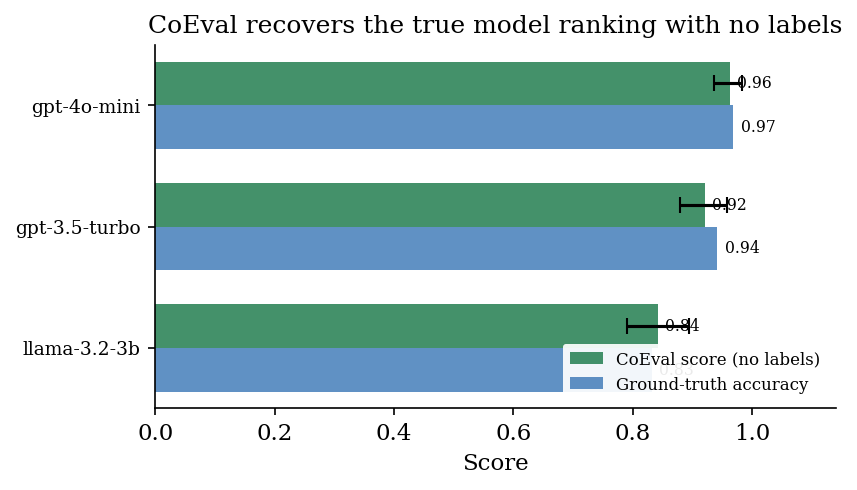
\includegraphics[width=\linewidth]{figures/f4_correctness_corr.png}
\caption{\textbf{Figure 1.} CoEval recovers the true model ranking with no labels. For each student model
the CoEval frontier-ensemble accuracy score (green, datapoint-clustered 95\% CI) and the held-out ground-truth
accuracy (blue) coincide within 0.02, and the order \texttt{gpt-4o-mini} \textgreater{} \texttt{gpt-3.5-turbo} \textgreater{}
\texttt{llama-3.2-3b} is reproduced exactly (cf. Table~2).}
\end{figure}

\begin{table}[tbp]
\centering
\small\setlength{\tabcolsep}{4pt}%
\caption{\textbf{Table 2.} CoEval reproduces the ground-truth model ranking. Three student models ranked by
CoEval frontier-ensemble accuracy score (datapoint-clustered 95\% CI) and by exact-match ground truth; the orderings
match.}
\setlength{\tabcolsep}{4pt}
\begin{tabularx}{\linewidth}{>{\hsize=1.022\hsize\raggedright\arraybackslash}X >{\hsize=0.989\hsize\raggedright\arraybackslash}X >{\hsize=0.989\hsize\raggedright\arraybackslash}X}
\toprule
Model under evaluation & CoEval score {[}95\% CI{]} & Ground-truth accuracy \\
\midrule
gpt-4o-mini & 0.963 {[}0.937, 0.984{]} & 0.969 \\
gpt-3.5-turbo & 0.921 {[}0.880, 0.958{]} & 0.942 \\
llama-3.2-3b & 0.843 {[}0.791, 0.895{]} & 0.832 \\
\bottomrule
\end{tabularx}
\end{table}

\textbf{Agreement with human judgments.} The validation above anchors the judge to objective exact-match
ground truth. We additionally test it against \emph{human} quality judgments on two standard meta-evaluation
benchmarks (Table~3), scoring with the same cheap cross-family panel (\texttt{gpt-4o-mini}, \texttt{claude-3.5-haiku},
\texttt{gemini-flash}). On SummEval \citep{ref37}, where experts rate machine summaries, the panel
correlates with human ratings at Spearman \(0.53\) (relevance), \(0.58\) (coherence), and \(0.56\) (consistency), in the
range strong single-model judges such as G-Eval \citep{ref2} report on this benchmark, reached here by a
panel of small models; the panel exceeds its best single judge on relevance and coherence, and the blind
single-judge average on all three. On LLMBar \citep{ref38}, which asks an evaluator to pick the
human-preferred output, the panel scores each output \emph{absolutely} (so no position bias) and prefers the
higher; it reaches \(0.845\) preference accuracy overall (\(0.94\) on the natural split), exceeding the expected accuracy
of a single judge chosen blind (\(0.76\)) by \(0.08\) and matching the best single judge (\(0.84\)) without needing to know
which judge that is. Because peer-agreement weights are near-uniform on a clean panel, the weighted and unweighted
panels coincide here; the weighting earns its value under judge-pool contamination (Section~5.2).

\begin{table}[tbp]
\centering
\small\setlength{\tabcolsep}{4pt}%
\caption{\textbf{Table 3.} Agreement with human judgments. CoEval cross-family panel versus humans on two standard
meta-evaluation benchmarks: SummEval (Spearman of panel score with expert ratings, \(n = 293\)) and LLMBar (accuracy
at matching the human-preferred output, \(n = 400\)). The panel tracks or exceeds the best single judge, which a
label-free user cannot select in advance, and clearly beats the blind single-judge average.}
\setlength{\tabcolsep}{4pt}
\begin{tabularx}{\linewidth}{>{\hsize=1.677\hsize\raggedright\arraybackslash}X >{\hsize=0.448\hsize\raggedright\arraybackslash}X >{\hsize=0.777\hsize\raggedright\arraybackslash}X >{\hsize=1.097\hsize\raggedright\arraybackslash}X}
\toprule
Benchmark and metric & Panel & Best single & Blind single (avg) \\
\midrule
SummEval relevance (Spearman) & 0.53 & 0.48 & 0.45 \\
SummEval coherence (Spearman) & 0.58 & 0.54 & 0.47 \\
SummEval consistency (Spearman) & 0.56 & 0.65 & 0.53 \\
LLMBar overall (accuracy) & 0.845 & 0.843 & 0.762 \\
~~LLMBar natural split (accuracy) & 0.941 & 0.860 & 0.831 \\
\bottomrule
\end{tabularx}
\end{table}

\subsection{Ensemble reliability: composition, judge-choice regret, and a self-validating panel}\label{ensemble-reliability-composition-judge-choice-regret-and-a-self-validating-panel}

The reliability of a judge ensemble is governed by its \emph{composition}, not its size. We measure average-measures
inter-rater reliability \(\mathrm{ICC}(3,k)\) as judges are added in descending order of agreement (Figure~2).
Reliability is \textbf{non-monotone}: a selected two-judge panel reaches \(\mathrm{ICC}(3,k) = 0.70\), but
appending lower-agreement judges \emph{lowers} it to \(0.45\) and then \(0.40\). This is the Spearman--Brown
relation (\hyperref[appA]{Appendix~A}) operating in reverse: an added judge with low mean correlation \(\bar{r}\) to the panel
reduces \(\bar{r}\) faster than the \(k\)-fold averaging can compensate, so the aggregate reliability \(R_k\) falls. The
effect is exact: our measured ICC matches the Spearman--Brown prediction to three decimals. Naively enlarging
a panel can therefore \emph{degrade} it; what matters is retaining high-agreement judges.

The decisive variable is \emph{composition}. Among the competent judges that CoEval\textquotesingle s consensus selection retains,
average-measures reliability follows the Spearman--Brown law: a selected two-judge panel already reaches
\(\mathrm{ICC}(3,k) = 0.70\). This is exactly why CoEval makes judge \emph{selection} a first-class step rather than
simply enlarging the panel: its
consensus criterion identifies and retains the high-agreement judges, delivering the reliable configuration
automatically. In other words, the framework converts panel composition from a liability for an unweighted
ensemble into a reliability \emph{gain}: the selected ensemble is robust to the inclusion of
weak models and more reliable than the unselected panel. The \(k\)-judge ensemble\textquotesingle s rank-agreement with the full-panel
consensus rises with \(k\) (Spearman \(\rho\): \(0.67, 0.74, 0.93, 1.00\)): a small selected panel already recovers most of
the full-panel ordering.

\begin{figure}[tbp]
\centering
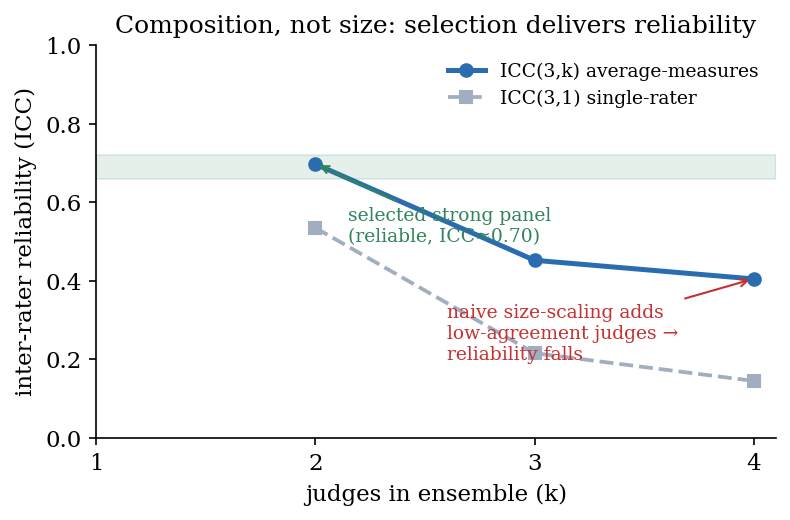
\includegraphics[width=\linewidth]{figures/f2_icc_curve.png}
\caption{\textbf{Figure 2.} Composition over size. Average-measures reliability ICC(3,~\emph{k}) as
judges are added in descending agreement order. A selected strong panel reaches ICC = 0.70; indiscriminately
adding low-agreement judges lowers the mean inter-rater correlation faster than averaging compensates, so reliability
falls. CoEval\textquotesingle s consensus selection retains the high-agreement judges, delivering the reliable configuration
automatically.}
\end{figure}

Composition matters because the \emph{wrong single judge can actively mislead}, and which judge is wrong is not
knowable a priori without the labels CoEval assumes are absent. Across the benchmark-grounded set of Section~5.1
(three tasks, \(n = 900\) pooled), the four candidate judges span a correlation range from \(-0.04\)
(\texttt{gpt-3.5-turbo}, anti-correlated) through \(0.17\) (\texttt{gemini-flash}) and \(0.24\)
(\texttt{gpt-4o-mini}) to \(0.31\) (\texttt{claude-haiku}): a \textbf{judge-choice regret of \(0.35\)}
between the best and worst single judge. The best judge is moreover task-dependent (\texttt{claude-haiku} here,
\texttt{gpt-4o-mini} on the summarization subset of Section~5.1), so a practitioner committing to one judge in
advance risks the anti-correlated one. The cross-family ensemble is the low-regret default: its plain mean correlates
at \(0.238\) and, unlike a single pick, is \emph{never} anti-correlated.

Given the panel, the choice of aggregator is itself a lever, and the unsupervised reliability-weighted aggregator of
Section~3.3 is the best label-free option we test. Weighting each judge by its agreement with the rest of the
panel assigns the anti-correlated \texttt{gpt-3.5-turbo} the lowest weight (\(0.18\) versus \(0.27\)--\(0.29\) for
the others) and lifts the aggregate correlation from the plain mean\textquotesingle s \(0.238\) to \textbf{\(0.246\)}. The
alternatives are worse: median and trimmed-mean aggregation, which discard rather than re-weight information, reach
only \(0.222\), and a Dawid--Skene latent-truth model \citep{ref33} over discretized scores reaches
\(0.178\). Reliability weighting
thus turns the panel\textquotesingle s own internal agreement, the one signal available without labels, into the strongest aggregate,
while never selecting the anti-correlated judge.

Aggregation does more than average: it lets the evaluator \emph{audit its own judges} with no labels. A judge\textquotesingle s mean
agreement with the rest of the panel is an unsupervised reliability signal, and it cleanly separates competent judges
from broken ones. We stress-test this by adding three deliberately broken judges to the four-judge panel, one returning
uniform-random scores, one a constant score, and one anti-correlated with quality. All three fall to the bottom of the
agreement ranking (mean agreement \(\le 0\) versus \(0.07\) to \(0.18\) for the competent judges), and their effect on a naive
average is large: the plain-mean correlation with ground truth drops from \(0.238\) to \(0.126\) once they are included.
Reliability weighting, using only peer agreement, assigns each broken judge a weight of essentially zero and recovers
the clean-panel accuracy (\(0.228\)). A single judge offers no such safeguard, because there is nothing to check it
against: the panel turns the absence of labels from a liability into a design that validates itself.

This self-correction has a precise boundary, and the boundary is exactly the cross-family design. It tolerates any
number of \emph{independent} broken judges: adding six uniform-random judges to the four-judge panel leaves the
reliability-weighted accuracy at \(0.25\) while the plain mean falls to \(0.16\), because independent noise never forms a
consensus to agree with. It fails only when a \emph{correlated} coalition of bad judges, all sharing one
systematic error, \emph{outnumbers} the competent judges: once five such judges face four good ones the coalition
becomes the apparent consensus, takes all the weight, and the recovered ranking inverts. Peer-agreement weighting is
therefore only as safe as the independence of judge errors, and \emph{vendor diversity is what supplies that
independence}: judges from distinct model families are unlikely to share a bias coalition. The robustness of the
aggregator and the cross-family composition principle are two sides of one design.

The panel\textquotesingle s two label-free quality signals, item discriminative power and judge agreement, compose into the
\emph{doubly-robust ranking} of Section~3.3, which leans on the items that separate models (Section~5.4)
and the judges that agree with the panel. On a benchmark-grounded check where gold accuracy is available (thirteen
models ranked on science QA and reasoning, spanning \texttt{gpt-4o} down to \texttt{llama-3.2-1b}), it improves
rank-recovery of the true model ordering from the plain mean\textquotesingle s Spearman \(0.88\) (Kendall \(0.76\)) to
\textbf{\(0.95\)} (Kendall \(0.87\)), by down-weighting saturated items that carry no ranking signal (nearly half
the items hold near-zero weight) and judges that disagree with the panel. The two signals are complementary, each
helping on its own (item-weighting alone \(0.94\), judge-weighting alone \(0.92\)) and most on the discriminative items
where judge reliability matters. The aggregator is robust: injecting a random judge degrades the plain mean to \(0.85\)
but leaves the doubly-robust ranking at \(0.95\), with the rogue judge receiving weight \(0.00\). Compared against standard
baselines on the same scores (Table~4), the doubly-robust ranking matches or beats the best single judge (an
oracle, since which judge is best is not knowable without labels), the unweighted panel (PoLL), and the median; its
decisive advantage is robustness to a contaminated judge pool: adding rogue judges steadily degrades the unweighted
mean (0.88, 0.85, 0.64) and even the median (0.94, 0.91, 0.71) at zero, one, and three rogue judges, while the
doubly-robust ranking is invariant to a minority rogue (0.95) and still leads at rogue parity (0.79).

\begin{table}[tbp]
\centering
\small\setlength{\tabcolsep}{4pt}%
\caption{\textbf{Table 4.} Rank-recovery on thirteen candidate models (science QA and reasoning; gold =
benchmark-native accuracy), comparing standard label-free baselines (best single judge, unweighted panel / PoLL,
median) against the CoEval weights. Each CoEval weight helps on its own, and the two compose into the best recovery;
the aggregator alone is robust to an injected random judge, which it gives weight 0.00. Values are the Spearman and
Kendall correlations between the recovered ranking and the gold-accuracy ranking.}
\setlength{\tabcolsep}{4pt}
\begin{tabularx}{\linewidth}{>{\hsize=1.888\hsize\raggedright\arraybackslash}X >{\hsize=0.582\hsize\raggedright\arraybackslash}X >{\hsize=0.530\hsize\raggedright\arraybackslash}X}
\toprule
Aggregator & Spearman & Kendall \\
\midrule
Best single judge (oracle) & 0.88 & 0.80 \\
Panel mean (PoLL) & 0.88 & 0.76 \\
Panel median & 0.94 & 0.88 \\
Item-weighted (discrimination) only & 0.94 & 0.84 \\
Judge-weighted (agreement) only & 0.92 & 0.82 \\
Doubly-robust (both) & 0.95 & 0.87 \\
~~with injected random judge: panel mean & 0.85 & 0.71 \\
~~with injected random judge: doubly-robust & 0.95 & 0.87 \\
\bottomrule
\end{tabularx}
\end{table}

The ensemble also cancels \emph{verbosity bias} (mixed-sign per-judge length biases average to a
near-zero ensemble correlation) and, by vendor-disjoint construction, precludes same-family
\emph{self-preference}; Appendix~E reports both, including the residual-bias measurements.

\subsection{Contamination resistance}\label{contamination-resistance}

We test the contamination-resistance claim empirically. We take the 400 CoEval-generated items from the
\texttt{medium-benchmark} study and measure their verbatim 13-gram overlap against a corpus of 491 items drawn
from five widely used public benchmarks (XSum, CNN/DailyMail, CodeSearchNet, SciQ, ARC-Challenge), datasets that
are, by virtue of their age and popularity, present in the pretraining corpora of current models. Across
\(110{,}784\) distinct public 13-grams, \textbf{not a single CoEval-generated item shares any 13-gram} with the
public corpus: mean and maximum overlap are both \(0.0000\), and \(0\%\) of generated items share any 13-gram. This
verbatim non-duplication \emph{corroborates} the structural guarantee: because items are synthesized fresh from the
attribute specification on each run, they cannot have appeared in any model\textquotesingle s \emph{prior} training, and a model
cannot retrieve them from a leaked copy of these widely-used benchmarks. (The scope from Section~5.1 holds: this
applies to CoEval\textquotesingle s generated items; the benchmark-grounded anchor of Table~1 deliberately reuses public items to
obtain objective ground truth.)

Non-duplication shows the items are fresh; a controlled study shows why that matters. We fine-tune a small open model
(Qwen2.5-0.5B) to memorize \(200\) public SciQ items, turning that public set into a contaminated benchmark, and compare
it against a clean frontier model (\texttt{gpt-4o-mini}) on both the memorized set and \(100\) fresh held-out items
of the same capability. On the contaminated benchmark the memorizer scores a perfect \(1.00\) and is ranked
\emph{above} \texttt{gpt-4o-mini} (\(0.845\)); on the fresh items the order is correct, with
\texttt{gpt-4o-mini} (\(0.81\)) above the memorizer (\(0.74\), its fresh-measured capability). The
memorized-minus-fresh gap isolates memorization from any skill the fine-tuning also imparted: the clean base model\textquotesingle s
gap is \(0.10\) (\(0.625\) vs \(0.53\)) while the contaminated model\textquotesingle s is \(0.26\) (\(1.00\) vs \(0.74\)), so \(0.16\) of its
apparent edge on the static benchmark is pure memorization that fresh items strip away. A static, possibly-contaminated
leaderboard thus ranks a \(0.5\)B memorizer ahead of a frontier model, an inversion that CoEval\textquotesingle s freshly-generated
items remove because no candidate can have trained on items synthesized after the fact.

\subsection{Putting it together: domain case studies}\label{putting-it-together-domain-case-studies}

We exercise the complete tool in its intended regime on three custom verticals,
\emph{drug--drug interaction reasoning}, \emph{clinical reasoning}, and \emph{legal analysis}, for
which we assume no task-specific labeled data and no trustworthy public benchmark. From a one-line description
each, CoEval generated 40 attribute-stratified items per vertical, three candidates answered, and the
cross-family panel scored every response, from one configuration file with no human labels. The panel produces
defensible rankings, a fully unanimous order on drug-interaction (\texttt{gpt-4o-mini} \(>\)
\texttt{gpt-3.5-turbo} \(>\) \texttt{llama-3.2-3b}, non-overlapping CIs) and consistent rankings on clinical
and legal, with \(71\%\) of generated items discriminative. Appendix~G reports the full results
(Table~G1) and Appendix~C the generated artifacts.

Rankings are also \emph{domain-specific}: across four de-novo domains three different models take first place,
so a generic leaderboard misdirects most practitioners. Appendix~D details this divergence (Table~D1).

\section{Discussion}\label{discussion}

CoEval is designed for a common predicament: ranking models for a task or domain when no labeled data exists and public
benchmarks cannot be trusted. The results show it meets that need, its label-free scores reproduce the true ranking,
track ground truth, and agree with human judgments (Section~5.1), and its items are verifiably fresh. The key
enabler is itself a contribution: the reliability of an LLM-judge panel is governed by its \emph{composition}, not its
size. A cross-family panel cancels the mixed-sign biases (verbosity, self-preference) any individual judge carries,
where a same-family panel would amplify a shared one, and a modest diverse panel already recovers most of the
full-panel reliability, so practitioners should prioritize vendor diversity over more copies of similar judges.

Coupling the panel to attribute-stratified generation makes CoEval more than a better judge: because items are
synthesized fresh on every run, it sidesteps contamination structurally rather than chasing leaked items, and targets
the deployment\textquotesingle s own distribution rather than a generic average. The same role separation that secures
contamination-freeness also precludes same-family self-preference, one architectural choice closing two leakage
channels, and a single declarative configuration regenerates the benchmark, responses, and scores.

\section{Conclusion}\label{conclusion}

We presented CoEval, a framework for \emph{ensemble self-evaluation} that ranks language models for a specific application when neither labeled data nor a trustworthy benchmark is available: from a task description alone, a pool of models rotates through all three roles, teacher, student, and judge, to generate a fresh, contamination-resistant benchmark, answer it, and rank the candidates, jointly weighting questions by discriminative power and judges by consensus, with no human annotation. Because every model also answers as a student, the same responses supply the data for both label-free weights. CoEval delivers
bias-cancelled, reliable evaluation without human annotation: it removes verbosity bias that no single judge avoids
(ensemble \(r = +0.010\), CI spanning zero; 93\% reduction), structurally precludes same-family self-preference, and
produces task-specialized rubrics with a shared quality core, while also converging
to a stable full-panel consensus (Spearman \(\rho\) up to \(1.00\)). Our
central finding, that judge-panel \emph{composition} rather than size is the decisive reliability lever, offers a
concrete and inexpensive recipe for trustworthy, renewable LLM evaluation.

The panel is also self-validating: because a
judge\textquotesingle s agreement with its peers is a label-free reliability estimate, the ensemble detects and zeroes out broken judges
with no ground truth, a safeguard a single judge cannot provide; the same weighting down-weights non-discriminative
challenges, so saturated questions carry no spurious ranking signal. Because model rankings are
\emph{domain-specific} (three different models top four de-novo domains, so a generic leaderboard misdirects most
practitioners) and the same declarative pipeline runs unchanged across models and domains, re-running on
every model release, CoEval is a reusable instrument a team points at its own application when neither labeled data nor
a trustworthy benchmark exists, rather than a single static study. CoEval is open-source and fully reproducible.

\section*{Limitations}\label{limitations}

Three boundary conditions delimit the validated regime. First, judge accuracy is anchored to objective exact-match QA,
where labels exist (Section~5.1, \(\rho = 0.86\)), and to human ratings on two public meta-evaluation benchmarks
(Section~5.1, SummEval and LLMBar); on the subjective custom domains (Section~5.4) the panel\textquotesingle s trustworthiness
rests on those anchors together with its measured bias and reliability properties (Section~5.2 and Appendix~E), and
rankings are reported as cross-family intervals rather than against a held-out gold ranking, which by assumption does
not exist. Task-specific human evaluation on those domains is the natural convergent check and the primary direction for
future validation. Second, the study spans up to thirteen candidate models across four exact-match QA tasks, three
custom verticals, a four-domain divergence study (Appendix~D), and a thirteen-model rank-recovery check
(Section~5.2); wider model pools and further domains would extend the evidence. Third, the contamination guarantee
is structural (fresh per-run synthesis), validated by zero verbatim overlap and a controlled memorization study
(Section~5.3); verbatim n-gram overlap and membership-inference probes such as Min-K\% \citep{ref36}
answer complementary questions, the former whether an item is reproduced, the latter whether it was seen during
pretraining.

\section*{Ethics Statement}\label{ethics-statement}

CoEval evaluates language models and involves no new human-subjects data collection. The human judgments used to
validate the judge (Section~5.1) come from existing public meta-evaluation benchmarks (SummEval, LLMBar) used
under their released licenses. The drug-interaction, clinical, and legal verticals (Section~5.4) are illustrations
of contamination-free benchmark generation, not validated decision-support systems, and should not be used for clinical
or legal decisions. Because CoEval generates evaluation items and scores them with language models, generated items and
rubrics can inherit model biases; the cross-family panel and the contamination checks mitigate but do not eliminate this
risk, and a practitioner applying CoEval in a high-stakes domain should pair it with human oversight.

\section*{Reproducibility}\label{reproducibility}

Every experiment is driven by a declarative configuration file and is reproducible end to end. The framework, the
canonical prompt templates (Appendix~C), the attribute and rubric specifications, the judge-panel definitions, and
the analysis code are released open-source, and the per-run scores and recovered rankings are recorded as artifacts. The
statistical estimators (ICC, bootstrap confidence intervals, the doubly-robust aggregator) are defined in
Appendix~A.



\begin{thebibliography}{99}
\setlength{\itemsep}{2pt plus 0.5pt}\setlength{\parsep}{0pt}
\bibitem[Butt et al.(2024)]{ref10}\label{r10} Butt, N., Awadalla, H., et al. (2024). BenchAgents: Automated Benchmark Creation with Agent
    Interaction. arxiv.org/abs/2410.22584 https://arxiv.org/abs/2410.22584
\bibitem[Chan et al.(2024)]{ref21}\label{r21} Chan, C.-M., Chen, W., Su, Y., et al. (2024). ChatEval: Towards Better LLM-based Evaluators through
    Multi-Agent Debate. ICLR. arxiv.org/abs/2308.07201 https://arxiv.org/abs/2308.07201
\bibitem[Chen et al.(2025)]{ref24}\label{r24} Chen, W.-L., Wu, Z., Bansal, H., et al. (2025). Do LLM Evaluators Prefer Themselves for a
    Reason? arxiv.org/abs/2504.03846 https://arxiv.org/abs/2504.03846
\bibitem[Chen et al.(2025)]{ref32}\label{r32} Chen, Y., et al. (2025). Recent Advances in Large Language Model Benchmarks against Data
    Contamination: From Static to Dynamic Evaluation. EMNLP. arxiv.org/abs/2502.17521 https://arxiv.org/abs/2502.17521
\bibitem[Dawid and P.(1979)]{ref33}\label{r33} Dawid, A. P., Skene, A. M. (1979). Maximum Likelihood Estimation of Observer Error-Rates Using
    the EM Algorithm. Journal of the Royal Statistical Society: Series C (Applied Statistics), 28(1), 20–28. doi.org/10.2307/2346806 https://doi.org/10.2307/2346806
\bibitem[Dubois et al.(2024)]{ref8}\label{r8} Dubois, Y., Galambosi, B., Liang, P., Hashimoto, T. B. (2024). Length-Controlled AlpacaEval: A Simple
    Way to Debias Automatic Evaluators. arxiv.org/abs/2404.04475 https://arxiv.org/abs/2404.04475
\bibitem[Fabbri et al.(2021)]{ref37}\label{r37} Fabbri, A. R., Kryściński, W., McCann, B., Xiong, C., Socher, R., Radev, D. (2021). SummEval: Re-evaluating Summarization Evaluation. Transactions of the Association for Computational
    Linguistics, 9, 391–409. arxiv.org/abs/2007.12626 https://arxiv.org/abs/2007.12626
\bibitem[Filice et al.(2025)]{ref31}\label{r31} Filice, S., Horowitz, G., Carmel, D., Karnin, Z., Lewin-Eytan, L., Maarek, Y. (2025). Generating
    Diverse Q\&A Benchmarks for RAG Evaluation with DataMorgana. SIGIR LiveRAG. arxiv.org/abs/2501.12789 https://arxiv.org/abs/2501.12789
\bibitem[Gu et al.(2024)]{ref19}\label{r19} Gu, J., Jiang, X., Shi, Z., et al. (2024). A Survey on LLM-as-a-Judge. arxiv.org/abs/2411.15594 https://arxiv.org/abs/2411.15594
\bibitem[Jain et al.(2025)]{ref23}\label{r23} Jain, N., Han, K., Gu, A., et al. (2025). LiveCodeBench: Holistic and Contamination Free Evaluation
    of Large Language Models for Code. ICLR. arxiv.org/abs/2403.07974 https://arxiv.org/abs/2403.07974
\bibitem[Kiela et al.(2021)]{ref14}\label{r14} Kiela, D., Bartolo, M., Nie, Y., et al. (2021). Dynabench: Rethinking Benchmarking in NLP. NAACL. arxiv.org/abs/2104.14337 https://arxiv.org/abs/2104.14337
\bibitem[Kim et al.(2024)]{ref3}\label{r3} Kim, S., Suk, J., Longpre, S., et al. (2024). Prometheus 2: An Open Source Language Model Specialized
    in Evaluating Other Language Models. arxiv.org/abs/2405.01535 https://arxiv.org/abs/2405.01535
\bibitem[Kim et al.(2025)]{ref7}\label{r7} Kim, S., Suk, J., Cho, J. Y., et al. (2025). The BiGGen Bench: A Principled Benchmark for Fine-grained
    Evaluation of Language Models with Language Models. NAACL. arxiv.org/abs/2406.05761 https://arxiv.org/abs/2406.05761
\bibitem[Li et al.(2024)]{ref9}\label{r9} Li, X. L., Kazemi, M., et al. (2024). AutoBencher: Towards Declarative Benchmark Construction. arxiv.org/abs/2407.08351 https://arxiv.org/abs/2407.08351
\bibitem[Li et al.(2025)]{ref20}\label{r20} Li, D., Jiang, B., Huang, L., et al. (2025). From Generation to Judgment: Opportunities and
    Challenges of LLM-as-a-Judge. EMNLP. arxiv.org/abs/2411.16594 https://arxiv.org/abs/2411.16594
\bibitem[Li et al.(2025)]{ref26}\label{r26} Li, Y., et al. (2025). Leveraging LLMs as Meta-Judges: A Multi-Agent Framework. arxiv.org/abs/2504.17087 https://arxiv.org/abs/2504.17087
\bibitem[Li et al.(2026)]{ref15}\label{r15} Li, D., Sun, R., Huang, Y., et al. (2026). Preference Leakage: A Contamination Problem in
    LLM-as-a-Judge. ICLR. arxiv.org/abs/2502.01534 https://arxiv.org/abs/2502.01534
\bibitem[Liu et al.(2023)]{ref2}\label{r2} Liu, Y., Iter, D., Xu, Y., et al. (2023). G-Eval: NLG Evaluation using GPT-4 with Better Human
    Alignment. EMNLP. arxiv.org/abs/2303.16634 https://arxiv.org/abs/2303.16634
\bibitem[Patel et al.(2025)]{ref30}\label{r30} Patel, A., Reddy, S., Bahdanau, D. (2025). CHASE: How to Get Your LLM to Generate Challenging
    Problems for Evaluation. arxiv.org/abs/2502.14678 https://arxiv.org/abs/2502.14678
\bibitem[Qian et al.(2026)]{ref27}\label{r27} Qian, C., Sun, G., Gales, M., Knill, K. (2026). Who can we trust? LLM-as-a-jury for Comparative
    Assessment. ICML. arxiv.org/abs/2602.16610 https://arxiv.org/abs/2602.16610
\bibitem[Raju et al.(2024)]{ref25}\label{r25} Raju, R., Jain, S., Li, B., et al. (2024). Constructing Domain-Specific Evaluation Sets for
    LLM-as-a-judge. arxiv.org/abs/2408.08808 https://arxiv.org/abs/2408.08808
\bibitem[Shashidhar et al.(2025)]{ref11}\label{r11} Shashidhar, S., et al. (2025). YourBench: Easy Custom Evaluation Sets for Everyone. arxiv.org/abs/2504.01833 https://arxiv.org/abs/2504.01833
\bibitem[Shi et al.(2024)]{ref36}\label{r36} Shi, W., Ajith, A., Xia, M., et al. (2024). Detecting Pretraining Data from Large Language
    Models. ICLR. arxiv.org/abs/2310.16789 https://arxiv.org/abs/2310.16789
\bibitem[Spiliopoulou et al.(2025)]{ref16}\label{r16} Spiliopoulou, E., et al. (2025). Play Favorites: A Statistical Method to Measure Self-Bias in
    LLM-as-a-Judge. arxiv.org/abs/2508.06709 https://arxiv.org/abs/2508.06709
\bibitem[Tan et al.(2025)]{ref6}\label{r6} Tan, S., Zhuang, S., Montgomery, K., et al. (2025). JudgeBench: A Benchmark for Evaluating LLM-based
    Judges. ICLR. arxiv.org/abs/2410.12784 https://arxiv.org/abs/2410.12784
\bibitem[Verga et al.(2024)]{ref5}\label{r5} Verga, P., Hofstatter, S., Althammer, S., et al. (2024). Replacing Judges with Juries: Evaluating LLM
    Generations with a Panel of Diverse Models (PoLL). arxiv.org/abs/2404.18796 https://arxiv.org/abs/2404.18796
\bibitem[Vu et al.(2024)]{ref4}\label{r4} Vu, T., Krishna, K., Alzubi, S., et al. (2024). Foundational Autoraters: Taming Large Language Models
    for Better Automatic Evaluation (FLAMe). EMNLP. arxiv.org/abs/2407.10817 https://arxiv.org/abs/2407.10817
\bibitem[Wang et al.(2024)]{ref34}\label{r34} Wang, Y., Yu, Z., Zeng, Z., et al. (2024). PandaLM: An Automatic Evaluation Benchmark for LLM
    Instruction Tuning Optimization. ICLR. arxiv.org/abs/2306.05087 https://arxiv.org/abs/2306.05087
\bibitem[Wataoka et al.(2024)]{ref18}\label{r18} Wataoka, K., Takahashi, T., Ri, R. (2024). Self-Preference Bias in LLM-as-a-Judge. arxiv.org/abs/2410.21819 https://arxiv.org/abs/2410.21819
\bibitem[White et al.(2025)]{ref22}\label{r22} White, C., Dooley, S., Roberts, M., et al. (2025). LiveBench: A Challenging, Contamination-Limited
    LLM Benchmark. ICLR. arxiv.org/abs/2406.19314 https://arxiv.org/abs/2406.19314
\bibitem[Xu et al.(2025)]{ref13}\label{r13} Xu, C., et al. (2025). Benchmark Data Contamination of Large Language Models: A Survey. arxiv.org/abs/2502.14425 https://arxiv.org/abs/2502.14425
\bibitem[Xu et al.(2026)]{ref29}\label{r29} Xu, C., Tan, Z., Wu, J., Zhou, T. (2026). A Judge-Aware Ranking Framework for Evaluating Large
    Language Models without Ground Truth. arxiv.org/abs/2601.21817 https://arxiv.org/abs/2601.21817
\bibitem[Ye et al.(2024)]{ref17}\label{r17} Ye, J., Wang, Y., Huang, Y., et al. (2024). Justice or Prejudice? Quantifying Biases in
    LLM-as-a-Judge. arxiv.org/abs/2410.02736 https://arxiv.org/abs/2410.02736
\bibitem[Zeng et al.(2024)]{ref38}\label{r38} Zeng, Z., Yu, J., Gao, T., Meng, Y., Goyal, T., Chen, D. (2024). Evaluating Large Language
    Models at Evaluating Instruction Following. ICLR. arxiv.org/abs/2310.07641 https://arxiv.org/abs/2310.07641
\bibitem[Zhang et al.(2024)]{ref12}\label{r12} Zhang, H., Da, J., Lee, D., et al. (2024). A Careful Examination of Large Language Model Performance on
    Grade School Arithmetic (GSM1k). arxiv.org/abs/2405.00332 https://arxiv.org/abs/2405.00332
\bibitem[Zhao et al.(2026)]{ref28}\label{r28} Zhao, Y., Shin, J., Huang, Z., Namburi, S., Sala, F. (2026). CARE: Confounder-Aware Aggregation
    for Reliable LLM Evaluation. arxiv.org/abs/2603.00039 https://arxiv.org/abs/2603.00039
\bibitem[Zheng et al.(2023)]{ref1}\label{r1} Zheng, L., Chiang, W.-L., Sheng, Y., et al. (2023). Judging LLM-as-a-Judge with MT-Bench and Chatbot
    Arena. NeurIPS. arxiv.org/abs/2306.05685 https://arxiv.org/abs/2306.05685
\bibitem[Zhu et al.(2023)]{ref35}\label{r35} Zhu, L., Wang, X., Wang, X. (2023). JudgeLM: Fine-tuned Large Language Models are Scalable
    Judges. arxiv.org/abs/2310.17631 https://arxiv.org/abs/2310.17631
\end{thebibliography}

% Appendices follow the bibliography (ACL/TACL convention). \appendix (added
% by pack when appendix.tex exists) restarts section numbering at A, B, C...
\appendix
\section{Statistical methods}\label{appA}

This appendix collects the estimator definitions used in the main text. CoEval reports the agreement of the judge
panel using intraclass correlation. For an average-measures design over \(k\) judges, the ICC(3,k) reliability is

\[\mathrm{ICC}(3,k) \;=\; \frac{MSR - MSE}{MSR},\]

where \(MSR\) is the between-targets (rows) mean square and \(MSE\) the residual mean square. The gain from aggregating
more judges follows the \textbf{Spearman--Brown} prophecy relation: if \(\bar{r}\) is the mean pairwise
inter-judge correlation, the reliability of a \(k\)-judge mean is

\[R_k \;=\; \frac{k\,\bar{r}}{1 + (k-1)\,\bar{r}}.\]

For categorical agreement (e.g., pass/fail rubric criteria) CoEval reports Cohen\textquotesingle s \(\kappa\),

\[\kappa \;=\; \frac{p_o - p_e}{1 - p_e},\]

where \(p_o\) is observed agreement and \(p_e\) the agreement expected by chance. To quantify residual bias and its
uncertainty, CoEval computes the Pearson correlation between a candidate confound (e.g., response length) and the
assigned score, with a \textbf{nonparametric bootstrap} confidence interval: the per-item (length, score)
pairs are resampled with replacement \(B\) times, the correlation is recomputed on each resample, and the
\(2.5\)th--\(97.5\)th percentiles of the bootstrap distribution form the reported 95\% CI. A CI that includes zero
indicates that the corresponding bias is statistically indistinguishable from absent. Across the family of correlation
tests reported in Section~5 we control the false-discovery rate with the Benjamini--Hochberg procedure
(\(\alpha = 0.05\)), and confidence intervals use a \emph{datapoint-clustered} resample wherever observations are
nested (multiple student responses per item).

\section{Rubric structure}\label{appB}

CoEval generates a scoring rubric automatically per task. We examine whether these rubrics are appropriately
task-specialized while sharing a common quality core. Across the four tasks, the 22 auto-generated rubric criteria
exhibit a mean \emph{within-task} semantic similarity of \(0.342\), exceeding the mean \emph{cross-task} similarity
of \(0.294\): criteria cluster by task, as desired. At the same time, a shared universal
\emph{``completeness''} dimension recurs across three of the four tasks, indicating a common quality core.
CoEval\textquotesingle s rubrics are thus specialized to each task\textquotesingle s demands yet anchored by a transferable notion of answer quality.

\begin{figure}[tbp]
\centering
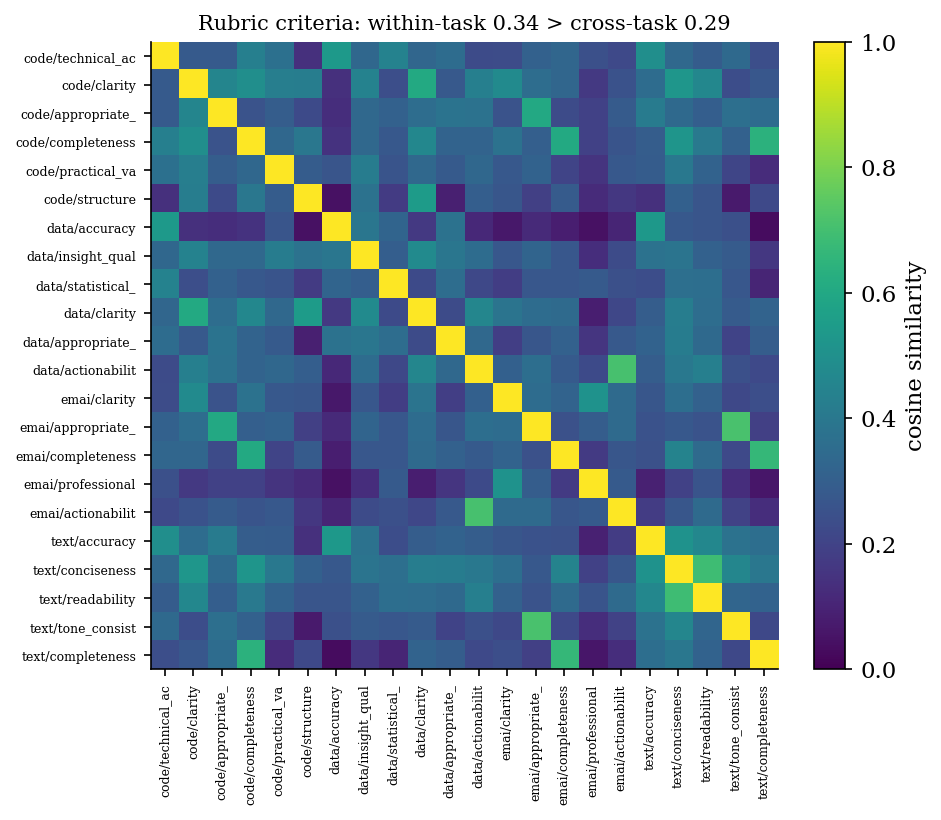
\includegraphics[width=\linewidth]{figures/f5_rubric_heatmap.png}
\caption{\textbf{Figure 3.} Pairwise semantic similarity of the 22 auto-generated rubric criteria across
four tasks. Block structure along the diagonal reflects task specialization (within-task 0.342 \textgreater{} cross-task
0.294), while a recurring ``completeness'' dimension forms a cross-task cluster.}
\end{figure}

\section{Worked examples on data-scarce domains}\label{appC}

The three verticals of Section~5.4 are domains where a practitioner typically has \emph{no} labeled
benchmark and no trustworthy public one: drug--drug interaction (DDI) reasoning, clinical decision support, and
legal analysis. The artifacts below are the \emph{actual} output CoEval generated for each, from a single one-line
task description and with no human labels. From that description the teacher inferred the attribute strata, synthesized
\(40\) contamination-free items stratified over them, and wrote a scoring rubric; the vendor-disjoint panel
(OpenAI~+~Anthropic~+~Google) then ranked three candidate models (Table~G1).

The pipeline is four templated calls to the teacher, all instantiated from the one-line
\texttt{task\_description} (and an optional \texttt{output\_description}). The first two build the attribute
space the items are stratified over; the third writes the rubric the panel scores against; the fourth generates one
contamination-free item per sampled attribute cell. The templates below are the verbatim framework prompts; a sampled
cell such as \emph{severity~=~moderate, mechanism~=~pharmacokinetic, patient\_context~=~pregnancy}
is what binds \texttt{\{target\_attributes\}} and yields the corresponding DDI item shown after Table~C1.

\textbf{(1) Target-attribute map.} Define the axes the benchmark varies over.

\begin{Verbatim}[breaklines=true,breakanywhere=true,fontsize=\small]
Generate synthetic data specifications for the {task_description} task by defining an
attribute space that characterizes possible outputs. Return a JSON object mapping each
attribute name to a list of possible values, and output only the JSON.
\end{Verbatim}


\textbf{(2) Nuance map.} Add surface-variation axes that change phrasing without changing the answer.

\begin{Verbatim}[breaklines=true,breakanywhere=true,fontsize=\small]
Define synthetic data specifications for the {task_description} task by creating a nuanced
variability-focused attribute space. Include only attributes that change document phrasing,
structure, noise, and context, without changing the underlying outputs. Return a single JSON
object mapping each attribute name to a list of allowed values, and output only the JSON.
\end{Verbatim}


\textbf{(3) Auto-rubric.} Write the task-specific scoring factors the judges apply.

\begin{Verbatim}[breaklines=true,breakanywhere=true,fontsize=\small]
For the task {task_description}, where the model's output is {output_description}, create an
evaluation rubric. Return only a JSON object where each key is a quality factor, and each
value is a concise description of that factor. Output only the JSON.
\end{Verbatim}


\textbf{(4) Item synthesis.} Generate one realistic item for a sampled attribute cell.

\begin{Verbatim}[breaklines=true,breakanywhere=true,fontsize=\small]
Generate a realistic benchmark data point.
Task: {task_description}
Output format: {output_description}
Required attributes: {target_attributes}
Nuance: {nuanced_attributes}

Return only a JSON object with exactly two string keys:
  "prompt":   a realistic input text for the task
  "response": the expected output for that input
Output only the JSON. No explanation or markdown.
\end{Verbatim}


Running this pipeline on the three one-line seeds below produces the auto-generated attribute strata and rubrics in
Table~C1, and the verbatim items that follow it.

\begin{table*}[t]
\centering
\small\setlength{\tabcolsep}{4pt}%
\caption{\textbf{Table C1.} From a one-line description to a scored benchmark, for three domains with no
public labeled data. The attribute strata and rubric criteria are auto-generated by the teacher; each domain yields
40 stratified, contamination-free items, scored by the cross-family panel.}
\setlength{\tabcolsep}{4pt}
\begin{tabularx}{\textwidth}{>{\hsize=1.214\hsize\raggedright\arraybackslash}X >{\hsize=1.193\hsize\raggedright\arraybackslash}X >{\hsize=0.593\hsize\raggedright\arraybackslash}X}
\toprule
Domain and one-line seed & Auto-generated attribute strata & Auto-generated rubric \\
\midrule
\textbf{Drug--drug interaction reasoning}\newline 
\emph{"given two or more co-administered drugs and a patient context, assess the interaction, its mechanism, severity, and clinical action"} & severity \{contraindicated, major, moderate, minor\}; mechanism \{pharmacokinetic, pharmacodynamic\};
patient\_\allowbreak{}context \{renal, hepatic, polypharmacy-elderly, pregnancy\} & interaction\_\allowbreak{}accuracy, severity\_\allowbreak{}correct, safety, completeness \\
\textbf{Clinical reasoning}\newline 
\emph{"a clinical reasoning question a clinician would face, requiring medical knowledge and safe, accurate reasoning"} & specialty \{cardiology, infectious\_\allowbreak{}disease, pediatrics, oncology, emergency\}; difficulty \{routine, intermediate, hard\} & clinical\_\allowbreak{}accuracy, safety, completeness, clarity \\
\textbf{Legal analysis}\newline 
\emph{"a legal analysis question requiring identification of the relevant rule and correct application to the facts"} & area\_\allowbreak{}of\_\allowbreak{}law \{contracts, torts, criminal, constitutional, intellectual\_\allowbreak{}property\}; complexity \{basic, intermediate, advanced\} & legal\_\allowbreak{}accuracy, reasoning\_\allowbreak{}quality, completeness, clarity \\
\bottomrule
\end{tabularx}
\end{table*}

One representative \emph{generated} item per domain (verbatim teacher output, labeled with its sampled attribute
cell), showing the synthesized items are specific and realistic rather than templated:

\begin{itemize}
\tightlist
\item
  \textbf{DDI} (severity = moderate, mechanism = pharmacokinetic, patient\_context = pregnancy):
  \emph{"A 30-year-old pregnant woman is prescribed lamotrigine for bipolar disorder and is also taking oral
  contraceptives. Assess the drug--drug interaction between these medications, identify the mechanism, and provide
  the severity and clinical recommendation."}
\item
  \textbf{Clinical} (specialty = cardiology, difficulty = routine):
  \emph{"A 62-year-old male with a history of hypertension and hyperlipidemia presents with progressive shortness of
  breath and occasional palpitations. On examination, you note elevated jugular venous pressure and a third heart
  sound. An ECG shows left ventricular hypertrophy. What is the most likely diagnosis and what initial management
  strategy should be considered?"}
\item
  \textbf{Legal} (area\_of\_law = torts, complexity = basic):
  \emph{"Alice, while jogging in the park, trips over a tree root that has been exposed due to erosion and falls,
  breaking her wrist. The park is owned by the city, and Alice claims the city is liable for her injuries due to
  negligence. Identify the relevant rule and determine if Alice can successfully hold the city liable."}
\end{itemize}

Each item is scored on its rubric by the panel, producing the rankings in Table~G1. On DDI the three judges are
unanimous, \texttt{gpt-4o-mini} (\(0.770\)) \textgreater{} \texttt{gpt-3.5-turbo} (\(0.682\)) \textgreater{}
\texttt{llama-3.2-3b} (\(0.497\)), with non-overlapping confidence intervals; on clinical reasoning the two stronger
models are statistically close (\(0.873\) vs \(0.864\)), which the overlapping intervals correctly expose. The entire path
from a one-line description to a defensible, contamination-free ranking is a single configuration file with no labeled
data and no human raters.

\section{Rankings are domain-specific: why a generic leaderboard misleads}\label{appD}

The case studies above rank models \emph{within} one domain. The premise of a custom-evaluation tool is that this
is necessary: the best model for one domain need not be the best for another, so a single public leaderboard, which
pools tasks into one number, can send a practitioner to the wrong model. We test this directly. From four one-line
descriptions, \emph{math word problems}, \emph{code explanation}, \emph{clinical reasoning}, and \emph{legal
analysis}, CoEval generated \(25\) contamination-free items each (\(100\) items), six candidate models answered them,
and the same vendor-disjoint cross-family panel (OpenAI~+~Anthropic~+~Google) scored every
response: \(1{,}800\) evaluations at full coverage, from one configuration file.

The four per-domain rankings \textbf{disagree sharply}. Three different models take first place across the four
domains, and each winner is stable under a bootstrap over items (\(B=2000\)): \texttt{gpt-4o-mini} tops clinical
reasoning (top with probability \(0.88\)) and code explanation (\(0.60\)), \texttt{gemini-flash} tops legal analysis
(\(1.00\)), and \texttt{claude-3.5-haiku} tops math word problems (\(0.85\)). The movement is not confined to the lead:
\texttt{gpt-4o-mini} falls from first on clinical reasoning to fifth of six on math (where it is top in only
\(0.001\) of bootstrap draws), and \texttt{claude-3.5-haiku} moves the opposite way, from first on math to fifth on
code (Table~D1). The mean cross-domain rank agreement is low (Kendall~\(\tau = 0.19\) averaged over the six
domain pairs); the least-aligned pair, code explanation versus math word problems, has a negative point estimate
(\(\tau = -0.41\)).

This is exactly the regret a generic leaderboard incurs. Pooling the four domains into one average ranks
\texttt{gemini-flash} first, but that model is the correct pick for only one of the four domains (legal analysis);
on clinical reasoning and code explanation the best model is \texttt{gpt-4o-mini}, and on math it is
\texttt{claude-3.5-haiku}, which the pooled board ranks only third. A practitioner who reads the generic
leaderboard and deploys its top model is choosing the domain-best model in just one of four cases. CoEval removes the
guess: it ranks the candidates on the practitioner\textquotesingle s own domain, contamination-free, with no labeled data.

\begin{table*}[t]
\centering
\small\setlength{\tabcolsep}{4pt}%
\caption{\textbf{Table D1.} The same six candidate models ranked by the same cross-family panel on four
CoEval-generated domains diverge: each cell is the model\textquotesingle s rank (1 = best) in that domain, rows ordered by the
generic pooled leaderboard. Three distinct models win the four domains (highlighted), and the pooled-best model
(\texttt{gemini-\allowbreak{}flash}) is domain-best in only one. \texttt{gpt-\allowbreak{}4o-\allowbreak{}mini} swings from 1st to 5th and
\texttt{claude-\allowbreak{}3.5-\allowbreak{}haiku} from 5th to 1st across domains.}
\small
\setlength{\tabcolsep}{4pt}
\begin{tabularx}{\textwidth}{>{\hsize=1.807\hsize\raggedright\arraybackslash}X >{\hsize=0.910\hsize\raggedright\arraybackslash}X >{\hsize=1.113\hsize\raggedright\arraybackslash}X >{\hsize=0.685\hsize\raggedright\arraybackslash}X >{\hsize=0.801\hsize\raggedright\arraybackslash}X >{\hsize=0.685\hsize\raggedright\arraybackslash}X}
\toprule
Model & Pooled & Clinical & Code & Legal & Math \\
\midrule
\texttt{gemini-\allowbreak{}flash} & 1 & 2 & 3 & 1 & 2 \\
\texttt{gpt-\allowbreak{}4o-\allowbreak{}mini} & 2 & 1 & 1 & 2 & 5 \\
\texttt{claude-\allowbreak{}3.5-\allowbreak{}haiku} & 3 & 3 & 5 & 3 & 1 \\
\texttt{qwen-\allowbreak{}2.5-\allowbreak{}7b} & 4 & 5 & 2 & 4 & 4 \\
\texttt{llama-\allowbreak{}3.1-\allowbreak{}8b} & 5 & 4 & 4 & 6 & 6 \\
\texttt{gpt-\allowbreak{}3.5-\allowbreak{}turbo} & 6 & 6 & 6 & 5 & 3 \\
\bottomrule
\end{tabularx}
\end{table*}

\section{Bias cancellation and cross-family self-preference}\label{appE}

We test whether the ensemble cancels verbosity bias (rewarding longer responses) on the four-task
\texttt{medium-benchmark} run. Per judge, length biases are of \emph{mixed sign}: \texttt{gpt-3.5-turbo}
penalizes length (\(r = -0.177\)), \texttt{smollm2-1.7b} rewards it (\(r = +0.234\)), with panel mean
\(\overline{|r|} = 0.153\) and no judge length-neutral (Table~E1). Averaging mixed-sign biases cancels
them: the \textbf{ensemble} length-score correlation is \(r = +0.010\) (95\% bootstrap CI \([-0.039,\, +0.057]\),
spanning zero), a 93\% reduction relative to the per-judge mean and statistically indistinguishable from length-neutral.
The cancellation comes from bias-sign diversity, which in this panel is correlated with vendor family, so vendor
diversity is a convenient, observable proxy for assembling judges whose idiosyncratic biases are unlikely to align.

\begin{table}[tbp]
\centering
\small\setlength{\tabcolsep}{4pt}%
\caption{\textbf{Table E1.} Verbosity bias (Pearson \emph{r} between response length and score) for representative
individual judges versus the CoEval ensemble. Individual judges carry length biases of opposite sign that the ensemble
cancels to a residual centered near zero.}
\setlength{\tabcolsep}{4pt}
\begin{tabularx}{\linewidth}{>{\hsize=1.041\hsize\raggedright\arraybackslash}X >{\hsize=1.000\hsize\raggedright\arraybackslash}X >{\hsize=0.959\hsize\raggedright\arraybackslash}X}
\toprule
Judge & Length-bias \(r\) & 95\% bootstrap CI \\
\midrule
gpt-3.5-turbo & -0.177 & n/a \\
SmolLM2 & +0.234 & n/a \\
Panel mean \(\overline{|r|}\) & 0.153 & n/a \\
CoEval ensemble & +0.010 & {[}-0.039, +0.057{]} \\
\bottomrule
\end{tabularx}
\end{table}

Recent work establishes that judge--generator relatedness inflates scores (\emph{Preference Leakage}
\citep{ref15}; \emph{Play Favorites} \citep{ref16}). CoEval addresses this \emph{structurally}:
requiring the judge panel to be vendor-disjoint from the student under test precludes any model from scoring its own
family, so a same-family preference cannot enter the aggregate at all, regardless of its magnitude on any individual
model.

Measured directly, the residual same-family preference is small and inconsistent in sign. Using
\texttt{gpt-4o-mini} as both a judge and a candidate in the verticals (Section~5.4), a difference-in-differences
that controls for a judge\textquotesingle s overall harshness gives \(+0.04\) on clinical reasoning (95\% CI \([-0.00, +0.08]\)), \(-0.04\) on
legal, and \(-0.04\) on drug-interaction: no systematic self-inflation survives. As an explicit safeguard,
\emph{vendor-disjoint aggregation} (when scoring a model, dropping any judge sharing its vendor family) leaves every
ranking in Table~2 and Table~G1 unchanged, with per-model scores shifting by at most \(0.016\), confirming the
cross-family rankings are already robust to same-family bias.

\section{System overview and experimental configuration}\label{appF}

\begin{figure*}[t]
\centering
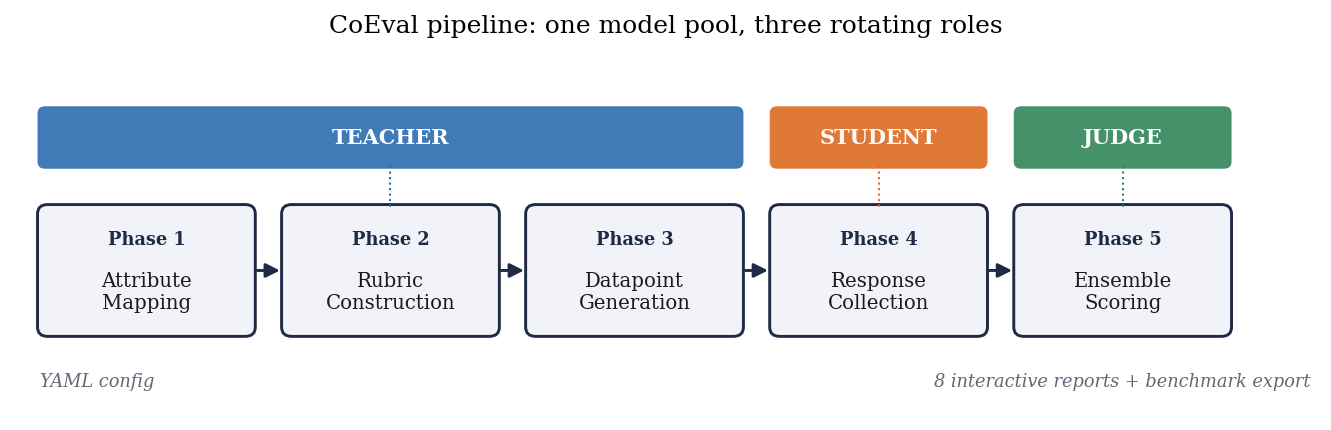
\includegraphics[width=\textwidth]{figures/f1_architecture.png}
\caption{\textbf{Figure 4.} The CoEval pipeline. A single pool of models rotates through three roles:
teachers map attributes, construct rubrics, and generate fresh benchmark items (Phases~1--3); students
produce candidate responses (Phase~4); and a cross-family judge ensemble scores them (Phase~5). The entire
run is specified in one declarative configuration.}
\end{figure*}

\begin{table*}[t]
\centering
\small\setlength{\tabcolsep}{4pt}%
\caption{\textbf{Table F1.} Experimental configurations. Judge panels differ by experiment: the
ground-truth anchor (Section~5.1) uses a frontier cross-family panel; the reliability and bias studies
(Section~5.2, Appendix~E) use a deliberately heterogeneous panel that includes weak open-weight judges;
and the verticals (Section~5.4, Appendix~D) reuse one fixed cross-family panel. All students are
gpt-4o-mini, gpt-3.5-turbo, and llama-3.2-3b unless noted.}
\setlength{\tabcolsep}{4pt}
\begin{tabularx}{\textwidth}{>{\hsize=0.920\hsize\raggedright\arraybackslash}X >{\hsize=1.067\hsize\raggedright\arraybackslash}X >{\hsize=1.272\hsize\raggedright\arraybackslash}X >{\hsize=0.742\hsize\raggedright\arraybackslash}X}
\toprule
Experiment & Task(s) & Judge panel & Size \\
\midrule
5.1 ground truth & SciQ, ARC (exact-match QA) & gpt-4o, claude-sonnet-4, gemini-2.5-flash & 191 items / 573 resp. \\
5.2 reliability (5.1 summ. anchor) & code (BLEU), news + text summ. (BERTScore) & gpt-4o-mini, gpt-3.5-turbo, claude-haiku, gemini-flash & 3 tasks / 900 resp. \\
5.2 + App.~E, App.~B & 4-task medium study & gpt-4o-mini, gpt-3.5-turbo, qwen2.5-1.5b, smollm2-1.7b & 7,978 eval. \\
5.4 verticals & drug-interaction, clinical, legal & claude-haiku, gemini-flash, gpt-4o-mini & 40 items each \\
5.3 contamination & SciQ memorization & exact-match (no LLM judge) & 200 memorized / 100 fresh \\
\bottomrule
\end{tabularx}
\end{table*}

\section{Domain case studies (full results)}\label{appG}

The preceding sections validate CoEval\textquotesingle s components where ground truth is available. We now exercise the complete tool
in its intended regime on three custom verticals, \emph{drug--drug interaction reasoning}, \emph{clinical
reasoning}, and \emph{legal analysis}, for which we assume no task-specific labeled data and no trustworthy
public benchmark. The drug-interaction vertical is the sharpest case for the framework\textquotesingle s premise: a well-known public
benchmark exists (DDIExtraction-2013) but is a relation-\emph{extraction} corpus rather than clinical-decision
reasoning, and is old and freely available enough to be presumed present in pretraining, while the few clinically
realistic DDI-reasoning sets are private and number only in the hundreds of items. From a one-line description per
vertical, CoEval\textquotesingle s teacher generated 40 attribute-stratified items (for drug interactions, stratified over severity,
mechanism, and patient context), three candidate models answered them, and the cross-family ensemble
(OpenAI~+~Anthropic~+~Google) scored every response, all from a single configuration file, with
no human labels or raters. \hyperref[appC]{Appendix~C} shows the actual generated artifacts for all three
domains: the one-line seed, the auto-generated attribute strata and rubric, and a representative synthesized item.

On the drug-interaction vertical CoEval produces a \textbf{clean, fully unanimous ranking}: all three
cross-family judges agree on the complete order \texttt{gpt-4o-mini}~(\(0.770\)) \(>\) \texttt{gpt-3.5-turbo}
~(\(0.682\)) \(>\) \texttt{llama-3.2-3b}~(\(0.497\)), with non-overlapping confidence intervals separating every
model (Table~G1). The clinical and legal verticals are consistent: the ensemble ranks the smallest model weakest in
both, unanimously in clinical and two-of-three in legal (where the Anthropic judge ranks \texttt{gpt-3.5-turbo}
lowest): genuine disagreement a single judge would hide and a diverse ensemble surfaces; on clinical the two
stronger models are statistically close, which the overlapping intervals correctly expose. This is the operation the
framework is built for: producing a defensible model ranking for a bespoke domain in which a standard benchmark is
unavailable or untrustworthy.

A ranking is only possible if the items \emph{separate} the models, the generation-side analog of judge
discrimination: a good teacher writes questions on which candidates actually differ. We measure per-item
discriminativeness as the spread of candidate-model ensemble scores. Across the \(120\) generated vertical items,
\textbf{\(71\%\) are discriminative} (a score range \(\ge 0.15\) across the three models), with a mean per-item
range of \(0.33\); on drug-interaction and legal analysis the figure rises to \(78\%\) and \(85\%\). Where the items do not
separate the models they are honest about it: clinical reasoning is only \(50\%\) discriminative precisely because its
two stronger candidates are genuinely close (\(0.873\) vs \(0.864\)), so the items reflect a real near-tie rather than
manufacturing a gap. This is why the panel yields non-overlapping ranking intervals: the teacher supplies items that
carry ranking signal, and a non-discriminative benchmark, on which every model scores alike, could not separate the
candidates no matter how reliable the judges are.

\begin{table}[tbp]
\centering
\small\setlength{\tabcolsep}{4pt}%
\caption{\textbf{Table G1.} CoEval ranks three candidate models on three custom, contamination-free verticals
generated from a task description with no labeled data. Scores are the cross-family ensemble mean ({[}0, 1{]}) with 95\%
bootstrap CI over 40 generated items. \texttt{llama-\allowbreak{}3.2-\allowbreak{}3b} ranks weakest in every vertical; the three judges
agree unanimously on the full drug-interaction order, unanimously on the weakest clinical model, and two-of-three in legal.}
\setlength{\tabcolsep}{4pt}
\begin{tabularx}{\linewidth}{>{\hsize=1.128\hsize\raggedright\arraybackslash}X >{\hsize=0.780\hsize\raggedright\arraybackslash}X >{\hsize=1.092\hsize\raggedright\arraybackslash}X}
\toprule
Vertical & Model & CoEval score {[}95\% CI{]} \\
\midrule
\emph{Drug--drug interaction} & gpt-4o-mini & 0.770 {[}0.739, 0.800{]} \\
& gpt-3.5-turbo & 0.682 {[}0.646, 0.717{]} \\
& llama-3.2-3b & 0.497 {[}0.459, 0.532{]} \\
\emph{Clinical reasoning} & gpt-3.5-turbo & 0.873 {[}0.849, 0.895{]} \\
& gpt-4o-mini & 0.864 {[}0.840, 0.885{]} \\
& llama-3.2-3b & 0.814 {[}0.784, 0.844{]} \\
\emph{Legal analysis} & gpt-4o-mini & 0.982 {[}0.973, 0.991{]} \\
& gpt-3.5-turbo & 0.740 {[}0.709, 0.770{]} \\
& llama-3.2-3b & 0.709 {[}0.677, 0.744{]} \\
\bottomrule
\end{tabularx}
\end{table}

\end{document}
